\chapter{CT RECONSTRUCTION}
\label{chap:reconstruction}

The essential goal of any reconstruction is to use the information gathered to estimate the parameters associated with the object.  In the case of CT, we use the information gathered on the detector over a range of angles to calculate the integral of the x-ray attenuation coefficients over the object voxels.  CT systems have evolved tremendously over the years, and reconstruction algorithms have also evolved dramatically to support the various types of systems. Over the years, reconstruction techniques have evolved using two general approaches to reconstruction: analytical and iterative.  In this chapter, we give a brief overview of these general techniques used for CT reconstruction, followed by an explanation of the method that was used for our system.

The first clinical CT scanner was installed in 1971 when it used a single detector and was dedicated to brain imaging only.  In 1973, a whole-body CT scanner was introduced~\citep{Ulzheimer2009}.  Up until 1990, most clinical CT scanners used the fan-beam geometry with axial rotation.  In the early 1990s, out of the desire to cover an entire human organ, the first single-slice helical/spiral CT scanner was introduced.  Ever since, spiral geometry became the main configuration for all clinical CT scanners.  Eliscint was the first to develop a two-slice CT system in the mid-1990s.  A few years later, General Electric (GE) came out with the first four-slice CT scanner and was quickly followed by all other major CT manufacturers.  The term multi-slice CT, also called multi-detector row CT (MDCT), quickly became the trend with manufacturers pushing for more, from 16 slices in 2002~\citep{Impact2002} to 320 slices in late 2007 by both Philips and Toshiba~\citep{Ulzheimer2009}.  The industry's push for larger volume coverage and faster scan time has fueled the need to develop newer and more efficient reconstruction algorithms.

\section{Analytic Reconstruction Techniques}

The most common method of image reconstruction for the earlier CT scanners was the fan-beam axial-filtered back-projection algorithm.  At the heart of the reconstruction algorithm is the Radon transform, which relates a function $f(\mathbf{r})$ to the collection of line integrals of that function $\lambda(p, \phi)$.  Shown in Eq.~\ref{eq:radon}, the projection line is described using $\mathbf{r \cdot \hat{n}} = p$, where $\mathbf{\hat{n}}$ is a unit vector making an angle $\phi$ to the x-axis, shown in Fig.~\ref{fig:RadonTransform}.  
%
\begin{equation}
\lambda(p, \phi) = \int_\infty d^2r \; f(\mathbf{r}) \delta(p- \mathbf{r} \cdot \mathbf{\hat{n}}).
\label{eq:radon}
\end{equation}

\begin{figure}[h]
\centering

\includegraphics[scale=1]{Radon_transform.eps}
\caption{2D Radon transform}
\label{fig:RadonTransform}
\end{figure}
%
To solve the Radon transform, the projection data on the detector at each angle go through a Fourier transform, which mathematically represents the object data in frequency space along the projection angle.  The Fourier transformed data are then filtered in the spatial frequency by a ramp filter, then back-projected into object space to reconstruct the original object.  This is also known as the Filtered Back-Projection (FBP) technique.  To solve for the fan-beam geometry, typically the projection data are gathered and rebinned into parallel sets before taking the inverse Radon transform to obtain the reconstructed slices.

CT scanning geometry can be divided into two general categories, depending on the targeted region of interest (ROI) within the body.  The first category is circular/axial orbit scanning, which is typically used to image smaller features of the body, such as a coronary artery, the brain, or the heart.  The circular-scanning geometry has the advantage of being very simple and fast, especially when the data acquired must be synchronized with a physiological signal, such as an EKG.  The most widely used reconstruction algorithm is the Feldkamp-Davis-Kress (FDK) reconstruction~\citep{Feldkamp1984}.  The algorithm is very similar to the conventional fan-beam reconstruction where the off-axis rays of the cone beam are weighted by a cosine term in order to approximate them as the 2D fan-beam rays.  The FDK algorithm works well when the cone angle is moderate, and many authors have proposed alternative methods to fix and compensate the image slices at the outer edges of the cone beam~\citep{Katsevich2003, Chen2003, Hu1996}.

The second and the most widely used scanning method is the helical/spiral geometry.  The approach to solve the helical cone beam reconstruction can be generally divided into two categories: approximate and exact reconstruction methods.  The most common method to solve this problem is the approximate reconstruction technique derived from the original FDK algorithm and later generalized to spiral scan by Ge Wang~\citep{Wang1993}.  Many authors have also succeeded in creating helical cone-beam algorithms based on the Feldkamp method~\citep{Wang1992, Kudo1991, Yan1992, Smith1992, Noo1999, Kachelriess2000, Tang2004, Tang2006a, Tang2006b}.  As noted by Wang, ``\textit{The key idea is to correct cone-beam data into fan-beam counterparts in a heuristic way.  As a primary example, a cone-beam datum along an oblique ray can be approximately converted to the fan-beam counterpart along a transverse ray by multiplying the former with the cosine of the angle between the oblique and transverse rays}''~\citep{Wang2007}.
%
\begin{figure}[h]
\includegraphics[width = 13cm]{Tam_figure.PNG}
\caption{Spiral-and-two-circles scan path for ROI imaging as proposed by Tam et al.~\citep{Tam1998}.}
\label{fig:tam_circle}
\end{figure}
%
Methods of solving for exact cone beam image reconstruction have been independently reported by Tuy, Smith, and Grangeat as early as 1983~\citep{Tuy1983, Smith1985, Grangeat1991}.  The requirement in all of these algorithms is that all the x-rays from the source that passes through the object must be covered by the detector.  For example in Tuy's condition, every plane that intersects with the object must also intersect with the x-ray source orbit at least once.  However, objects in medicine and many industrial inspections are very long, which would require a very large area detector to cover the entire length of the object.  In addition, in most of these objects, only a smaller section is of interest.  The problem of solving for a smaller ROI without scanning the entire object is extremely challenging.  Intuitively, we need to collect all of the x-ray paths that penetrate the ROI for reconstruction.  However, because parts of these x-ray beams are ``corrupted'' by other parts of the objects, they no longer represent the ROI exclusively.  We can attempt to solve the ``corrupted'' parts of the x-ray paths, but the data are often missing because the detector was not large enough to collect all of the information.  This problem is known as data truncation, or missing data.  The method of solving the exact solution to an long object problem with a ROI was proposed by Tam in 1998 using a spiral-and-two-circle scan path for ROI imaging~\citep{Tam1998}, as shown in Fig.~\ref{fig:tam_circle}.  Unfortunately, it is not entirely trivial to merge the truncated data from multiple helical turns,  which would also increase radiation dose and scan time.  This problem was not solved until early 2002 by Katsevich's breakthrough~\citep{Katsevich2002SIAM, Katsevich2003, Katsevich2004}.
%
%\begin{figure}[h]
%	\begin{subfigure}[b]{0.2\linewidth}
%		\includegraphics[scale=0.7]{circle-plus-line.eps}
%		\caption{}
%		\label{fig:circle-line}
%	\end{subfigure}
%	\begin{subfigure}[b]{0.2\linewidth}
%		\includegraphics[scale=0.7]{circle-plus-arc.eps}
%		\caption{}
%		\label{fig:circle-arc}
%	\end{subfigure}
%	\begin{subfigure}[b]{0.2\linewidth}
%		\includegraphics[scale=0.7]{dual-circle.eps}
%		\caption{}
%		\label{fig:dual-circle}
%	\end{subfigure}
%	\begin{subfigure}[b]{0.2\linewidth}
%		\includegraphics[scale=0.7]{saddle.eps}
%		\caption{}
%		\label{fig:saddle}
%	\end{subfigure}
%\caption{Different scanning trajectories for complete sampling. \ref{fig:circle-line}: circle-plus-line, \ref{fig:circle-arc}: circle-plus-arc, %\ref{fig:dual-circle}: dual circle, and \ref{fig:saddle}: saddle}
%\label{fig:scanning_trajectories}
%\end{figure}
%
\begin{figure}[h]
\includegraphics[scale=1]{scanning_trajectories}
\caption{Different scanning trajectories for complete sampling. (a) circle-plus-line; (b) circle-plus-arc; (c) dual circles; and (d) saddle.}
\label{fig:scanning_trajectories}
\end{figure}

Since Katsevich's invention, various sophisticated formulas have been proposed and developed for exact reconstruction using longitudinally and transversely truncated projection data and for various scanning geometries shown in Fig.~\ref{fig:scanning_trajectories}.  However, although these algorithms are highly sophisticated and novel, they are computationally expensive compared to the popular FBP algorithms, not to mention the difficulties in building the hardware.  Currently, most CT manufacturers still use the approximate cone-beam reconstruction algorithms instead of exact cone-beam reconstruction algorithms for two reasons.  First, the data requirements for exact reconstruction are still too difficult due to physical constraints.  Second, the approximate algorithms already provide very good and sometimes even better performance compared to the exact reconstruction method, which may not have the best noise characteristics~\citep{Wang2008}.  It will be interesting to see when exact algorithms will replace approximate algorithms in the future.

\section{Iterative Reconstruction Techniques}
Iterative reconstruction techniques attempt to solve for the object using projection images in an iterative fashion, where the solution to the object at the current iteration will be used for the next iteration.  All iterative reconstruction methods consist of three major steps, which are repeated iteratively until a final solution is reached.  First, a forward projection of the object creates an estimate of the raw data.  Second, the estimated raw data and the real measured data are compared, and a correction term is calculated.  Third, the correction term is back-projected onto the object to create a new estimate of the object.  Shown in Fig.~\ref{fig:generalIR}, this process is repeated until either a fixed number of iterations is reached or the object estimation reaches a predefined criterion.
%
\begin{figure}
\centering
\includegraphics[scale = 0.9]{iterative_recon_process.eps}
\caption{The general process of iterative algorithm~\citep{Beister2012}.}
\label{fig:generalIR}
\end{figure}

\subsection{Algebraic Iterative Reconstruction Techniques}
From a historical perspective, the very first reconstructed CT image was created using the algebraic iterative reconstruction (ART) method, where the method attempts to find the object by solving a series of linear equations,
%
\begin{equation}
\mathrm{A\,\mathbf{x} = \mathbf{b}}.
\label{eqn:art}
\end{equation}.  
%
In terms of image reconstruction, the elements of $\mathrm{\mathbf{x}}$ are the object voxel values that need to be reconstructed, $\mathrm{A}$ is the system matrix that models the production of the image data, and the elements of $\mathrm{\mathbf{b}}$ are the pixels values of the measured raw data.  The entries of the matrix $\mathrm{A}$ correspond to x-rays from the source through the object volume to the detector pixels.  Solving for the object voxel values involves solving for Eqn~\ref{eqn:art}, where $\mathrm{A}$ is most likely not a square matrix and fairly large in size.  Starting from ART, a series of algorithms evolved that would try to converge to the solution faster, reduce noise, and reduce problems with streak artifacts; however, in general, all ART-based methods are non-statistical and model the geometry of the acquisition process better than common analytical methods based on FBP.  Therefore, ART-based methods can better deal with sparse data and an irregular sampling of acquisition positions~\citep{Beister2012}.

\subsection{Statistical Iterative Reconstruction Techniques}
Statistical iterative reconstruction techniques have been used extensively in single photon emission tomography (SPECT) and positron emission tomography (PET), where low photon rates and noise are major issues.  Since the increase in public awareness of CT radiation and the need to reduce the risks associated with radiation, transitioning to statistical iterative reconstruction techniques has the potential of lowering radiation doses while suppressing image noise from low-dose scan techniques.  Therefore, it is crucial that the mathematical models of the CT system are accurate, and the modeling errors are suppressed so they do not grow to during the iterative process.  There are two types of models that are typically used in iterative reconstruction algorithms: a physical model that involves the geometry of the system and a statistical model that attempts to formulate the noise within the imaging system.

%The physical model of the CT system can account for any physical process and is only limited by the computational power of the processing computer.  Unlike analytical reconstruction techniques where numerous physical assumptions were made to allow for the mathematics to be manageable, where the size of the x-ray focal spot is assumed to be infinitely small; the shape and dimension of the detector cells were ignored; and all x-ray photon interactions were assumed to take place at the center of the detector cell.

Unlike the analytical reconstruction techniques, where many physical assumptions must be made to allow for the mathematics to be more manageable, physical models used by the iterative algorithm can account for any physical process and are only limited by the computational power of the processing computer.  For example, analytical solutions usually assume that the x-ray focal spot is infinitely small; the shape and dimension of the detector cells are ignored so that all x-ray photon interactions were assumed to take place at the center of the detector cells.  Iterative reconstruction algorithms require no prior assumption about the geometry of the system.  For example, a commonly used model is to cast multiple pencil rays through the x-ray focal spot, the image voxel, and the detector pixel to mimic different x-ray photon paths through the object.  The summation of the x-rays at each detector cell is then used to approximate the CT image system, shown in Fig.~\ref{fig:physical_modeling}a. Needless to say, this method is extremely time-consuming and computationally intensive.  Another commonly used approach is to model the ``shadow'' cast by each image voxel onto the detector cells and rely on the point-response function to model the forward projection process of the CT system, where the response function is non-stationary and changes with the voxel location to account for different magnifications and orientations, shown in Fig.~\ref{fig:physical_modeling}b.  Comparatively, this method is computationally more efficient~\citep{Hsieh2013}.
%
\begin{figure}
\includegraphics[scale=1]{ct_IR_model}
\caption{Common physical models used for the iterative reconstruction algorithm. (a) the pencil beam model; and (b) the point-response model.}
\label{fig:physical_modeling}
\end{figure}

The statistical model or the noise model attempts to incorporate the statistics of the detected photon into the reconstruction process.  This may include incident photon flux variations, also known as the Poisson distribution, though it is approximate due to the poly-energetic x-ray source used in CT, the energy-dependent light production in the scintillator, shot noise in photodiodes, and electronic noise in readout electronics. The most common noise model is the zero-mean Gaussian noise.

Once both the geometry and noise of the CT system are properly modeled.  A cost function is chosen.  The iterative process searches for the minimum of the cost function, and the solution that minimizes this cost function is the reconstructed object.  This cost function, sometimes called an objective functional, typically consists of two components: a data agreement term that evaluates the difference between the experimental data and the data generated by the model, and a regularizing term, sometimes called a penalty function that depends only on the object and serves as a prior, such as positivity.  If the functional is strictly convex, then the minimum is unique, and all algorithms should obtain the same image if they were to run to convergence.  The only decision will be to looking for an algorithm that will find the minimum of the functional using the least amount of computing resources.  In practice, however, iterative algorithms may not be run to convergence, and the resulting image depends on the algorithm, the initial estimate, and the stopping rule.

\section{Maximum-Likelihood Expectation-Maximization (MLEM) algorithm }
In this project, we used the Maximum-Likelihood Expectation-Maximization algorithm for the reconstruction process without any regularization functions.  The MLEM algorithm is shown in Eq.~\ref{eq:MLEM}~\citep{EmissionTom2004}, where $g_i$ are the image pixel values for all projection angle and represent the attenuation values of x-rays through the object voxels onto each detector pixels, $H_{ij}$ is the imaging matrix that models the x-ray imaging system and maps the object voxel value to image pixel value, and $f_{j}$ are the object voxel values, and represent the x-ray attenuation coefficient of the object integrated over the object voxel.
%
\begin{equation}
\hat{f}^{(n+1)}_{j} = \frac{\hat{f}^{(n)}_j}{{\sum\limits_{i'}} \, H_{i'j}} \; 
						\sum\limits_{i} H_{ij} \, \frac{g_{i}}{\sum\limits_{k} \, H_{ik} \hat{f}_{k}^{(n)}}
\label{eq:MLEM}
\end{equation}
%
$\sum\limits_k h_{ik} \hat{f}_k^{(n)}$ takes the current object voxel values, $\hat{f}^{(n)}_k$, and calculates its forward projection image at all angles.  The forward projection images are then divided into the data image vector, $g_i$, for every angle.  The result, $\frac{g_i}{\sum\limits_k H_{ik} \hat{f}_k^{(n)}}$, is a ratio between the set of simulated projection images and the experimental data.  This ratio is then back-projected into object space.  The next iteration for object voxels, $\hat{f}_j^{n+1}$, is calculated by multiplying the back-projected ratio by the current object voxel values, $\hat{f}_j^{(n)}$, and scaled by the sensitivity $S_j$.  The sensitivity , $S_j = \sum\limits_{i'} \, H_{i' j}$, is calculated by summing the $H$ matrix over all detector pixels and projection angles, which represents the back projection of the detector values from all projection angles onto the object voxel values.

The most important factor in the MLEM algorithm is the imaging matrix, $H$, that models the imaging system.  Typically, the $H$ matrix is modeled in PET or SPECT system and the reconstruction is performed using a FBP algorithm.  Or the $H$ matrix can be measured, where a point source is scanned throughout the entire volume of the object, and signals are recorded for every object point at every detector pixel for all detectors.  To re-create this for CT is nearly impossible because the $H$ matrix would have been astronomically large due to the number of detector pixels and projection angles.  Instead of using a stored $H$ matrix, we opted to model the CT system and compute the $H$ matrix as operators by calculating the forward projection and backward projection processes on-the-fly using a Graphics Processing Unit (GPU).

\section{CT model and projector calculation}
The pencil beam model was used for both the forward and backward projection process, where we assumed that each x-ray beam is launched from an infinitely small x-ray point source. This pencil beam travels towards the geometrical center of each detector pixel.  Along the way, the contributions from every voxel for each ray is calculated according to Siddon's algorithm~\cite{Siddon1985}.  This model does not account for any scatter in the object and it assumes that the x-ray beam is monochromatic.
%
\begin{figure}[h]
\centering
\includegraphics[scale=1]{voxel_projection.eps}
\caption{The (a) forward and (b) backward projection process.}
\label{fig:voxel_projection}
\end{figure}

In the forward projection process, the final value at the each of the detector element represents the summation of the product between the length of the ray that passed through each voxel and the value at each voxel, shown in Fig.~\ref{fig:voxel_projection}a.  In the backward projector, the order is reversed. We take the value at the detector element, trace a ray backward through the object volume to the x-ray source.  For every voxel penetrated by that ray, we calculate the section of the ray that passed through a voxel and multiply this length by the value at the detector element, shown in Fig.~\ref{fig:voxel_projection}b.  This process was repeated for all x-rays, i.e., all detector pixels.

In the next section we will explain briefly the Siddon's algorithm and how we modified the algorithm so it can be implemented on the GPU. 

\subsection{Siddon's algorithm}
%
\begin{figure}
\centering
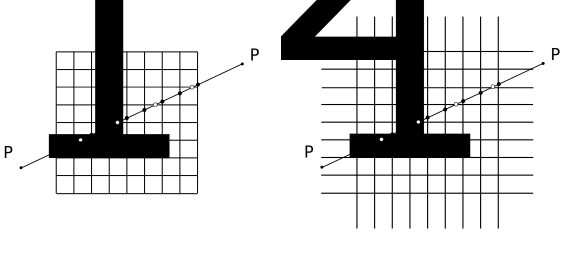
\includegraphics[scale=0.8]{siddon_proj_planes.eps}
\caption{Considering a 2-dimensional object (a) as the intersection areas of orthogonal sets of equally spaced, parallel lines (b).}
\label{fig:forward_backward_model}
\end{figure}
%
The Siddon's algorithm is a method of calculating the exact radiological path for a three-dimensional voxel array.  Instead of directly calculating the intersections of the ray with each pixel, it calculates the ray's intersection with three parallel planes in the object volume $\{ x, y, z \}$.  For simplicity, a 2-dimensional object is shown in Fig.~\ref{fig:forward_backward_model}.  In the figure, the intersection of the ray with equally spaced, parallel lines is a very simple problem.  Since the lines are equally spaced, it is only necessary to determine the first intersection.  The other intersections can then be automatically generated by recursion.  

For a 3-dimensional CT volume array of $(N_x -1, N_y-1, N_z-1)$ voxels, the orthogonal sets of equally spaced, parallel planes can be written as,
%
\begin{equation}
	\begin{aligned}
		X_{plane}(i) & = X_{plane}(1) + (i-1)\, d_x 	&(i = 1, ..., N_x),\\ 
		Y_{plane}(j) & = Y_{plane}(1) + (j-1)\, d_y  	&(j = 1, ..., N_y),\\
		Z_{plane}(j) & = Z_{plane}(1) + (k-1)\, d_z		&(k = 1, ..., N_z),
	\end{aligned}
	\label{eq:siddon_planes}
\end{equation}
%
where $d_x$, $d_y$, and $d_z$ are the distances between the $x$, $y$, and $z$ planes, respectively.  They are also the lengths to the sides of the volume voxel.  We can calculate a ray's intersection with the initial and final planes of the volume array, initiating at the point, $P_1 = (X_1, Y_1, Z_1)$, and terminating at the point, $P_2 = (X_2, Y_2, Z_2)$, by first calculating a set of minimum and maximum parametric values for that ray using the following equation,
%
\begin{equation}
\begin{aligned}
\alpha_x(1) &= \frac{X_{plane}(1) - X_1}{X_2 - X_1}, \qquad &\alpha_x(N_x) &= \frac{X_{plane}(N_x) - X_1}{X_2 - X_1}, \\
\alpha_y(1) &= \frac{Y_{plane}(1) - Y_1}{Y_2 - Y_1}, \qquad &\alpha_y(N_y) &= \frac{Y_{plane}(N_y) - Y_1}{Y_2 - Y_1}, \\
\alpha_z(1) &= \frac{Z_{plane}(1) - Z_1}{Z_2 - Z_1}, \qquad &\alpha_z(N_z) &= \frac{Z_{plane}(N_z) - Z_1}{Z_2 - Z_1}. \\
\end{aligned}
\label{eq:siddon_alpha_extremes}
\end{equation}
%
If the denominator, $(X_2 - X_1)$, $(Y_2-Y_1)$, or $(Z_2 - Z_1)$ is equal to zero, then the ray is parallel to that particular plane, and the corresponding $\alpha_x$, $\alpha_y$, or $\alpha_z$ will be undefined and excluded from the calculation.  These equations calculates the surface planes of the CT volume against the initial and final points of the ray, as shown in 2-dimensions in Fig.~\ref{fig:siddon_intersection_planes}.
%
\begin{figure}[ht]
\centering
\includegraphics[scale=1.5]{siddon_projection_intersection_planes.eps}
\caption{Siddon's algorithm showing the minimum and maximum parametric values for a ray passing through a 2D object array.}
\label{fig:siddon_intersection_planes}
\end{figure}

Once the values from Eq.~\ref{eq:siddon_alpha_extremes} is found, two parametric values that are used to indicate the initial and final intersection of the ray with the object volume is determined using,
%
\begin{equation}
\begin{aligned}
\alpha_{min} = \; & max\{ 0, \, min \left[ \alpha_x(1), \, \alpha_x(N_x) \right], \\
               & \; \; \; \; min \left[ \alpha_y(1), \alpha_y(N_y) \right], min \left[ \alpha_z(1), \alpha_z (N_z) \right] \}, \\
\alpha_{max} = \; & min\{1, \, max \left[ \alpha_x(1), \, \alpha_x(N_x) \right], \\
			   & \; \; \; \; max \left[ \alpha_y(1), \alpha_y(N_y) \right], max \left[ \alpha_z(1), \alpha_z (N_z) \right] \}.
\end{aligned}
\label{eq:siddon_alpha_min_max}
\end{equation}
%
If $\alpha_{max}$ is less than or equal to $\alpha_{min}$, then the ray does not intersect the object volume and that ray will be excluded from the calculation.  $\alpha_{min}$ and $\alpha_{max}$ are scaled against the total distance between $P_1$ and $P_2$, and are valued between 0 and 1.

Once we have determined the intersections of the ray with the surface planes of the object volume, we can then calculate the plane indices that will be intersected by the ray inside the object volume using the following equations, 
%
\begin{equation}
	\begin{aligned}
	\text{if $ (X_2 - X_1) \geq 0 $ }\\
	i_{min} &= N_x - \left[ X_{plane}(N_x) - \alpha_{min} (X_2 - X_1) - X_1 \right] /  d_x, \\
	i_{max} &= 1 + \left[ X_1 + \alpha_{max} (X_2 - X_1) - X_{plane}(1) \right] / d_x. \\
	\text{if $ (X_2 - X_1) \leq 0 $ }\\
	i_{min} &= N_x - \left[ X_{plane}(N_x) - \alpha_{max} (X_2 - X_1) - X_1 \right] /  d_x, \\
	i_{max} &= 1 + \left[ X_1 + \alpha_{min} (X_2 - X_1) - X_{plane}(1) \right] / d_x, 
	\end{aligned}
\label{eq:siddon_ijkminmax}
\end{equation}
%
and with similar expressions for $j_{min}$, $j_{max}$, $k_{min}$, and $k_{max}$.  Note that values when $(X_2 - X_1) = 0$, $(Y_2 - Y_1) = 0$, and $(Z_2 - Z_1) = 0$ had been excluded from these calculations.  The indices are rounded towards nearest integer though care must be taken when calculating the indices near the object surface planes.  In execution, both the upper and lower bound integers were calculated and the actual indices were selected based on the values of $\alpha_{min}$ and $\alpha_{max}$.  Then, the corresponding parametric values to each index are computed using,
%
\begin{equation}
\begin{aligned}
\alpha_x(i) &= [ X_{plane}(i) - X_1 ] / (X_2 - X_1) \\
			&=\alpha_x(i-1) + d_x / (X_2 - X_1) \,
\end{aligned}
\label{ea:siddon_alphas}
\end{equation}
%
with similar expressions for $\alpha_y$, and $\alpha_z$.  

Once the set of parametric values $\{\alpha_x\}$, $\{\alpha_y\}$, and $\{\alpha_z\}$ for the ray are calculated, we can then determine the length of the ray that passed through a voxel by first merge the parametric values into one large set as, $\{ \alpha \}  = \{ \{\alpha_x\}, \{\alpha_y\}, \{\alpha_z\} \}$, and sort $\{ a \}$ in ascending order from the lowest to the highest value.  The path length through a voxel can then be calculated using, 
%
\begin{equation}
l(m) = d_{12} \left[ \alpha(m) - \alpha(m-1) \right] \qquad (m = 1, ..., n),
\label{eq:siddon_length}
\end{equation}
%
where the quantity $d_{12}$ is the distance between $P_1$ and $P_2$, and is determined by,
%
\begin{equation}
d_{12} = \left[ (X_2 - X_1)^2 + (Y_2 - Y_1)^2 + (Z_2 - Z_1)^2 \right]^{1/2}, 
\label{eq:siddon_d12}
\end{equation}
%
and $n$ is the number of elements in the set $\{ a \}$,
%
\begin{equation}
n = (i_{max} - i_{min} + 1) + (j_{max} - j_{min}+1) + (k_{max}-k_{min}+1) + 1.
\label{eq:siddon_n}
\end{equation}
%
\begin{figure}[ht]
\centering
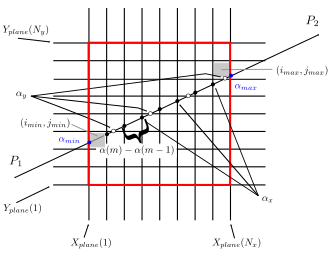
\includegraphics[scale= 1.5]{siddon_proj_planes_detail.eps}
\caption{A detailed view of the variables for the Siddon's algorithm in 2-dimensions.}
\label{fig:siddon_plane_detail}
\end{figure}
%
This calculation is graphically represented in Fig.~\ref{fig:siddon_plane_detail} in 2-dimensions.

To locate the particular voxel index, $i(m), j(m), k(m)$, bounded by $\alpha_{m-1}$ and $\alpha_m$, we can use the following equation,
\begin{equation}
\begin{aligned}
i(m) &= 1 + \left[ X_1 + \alpha_{mid}(X_2 - X_1) - X_{plane}(1) \right] /d_x, \\
j(m) &= 1 + \left[ Y_1 + \alpha_{mid}(Y_2 - Y_1) - Y_{plane}(1) \right] /d_y, \\
k(m) &= 1 + \left[ Z_1 + \alpha_{mid}(Z_2 - Z_1) - Z_{plane}(1) \right] /d_z,
\end{aligned}
\label{eq:siddon_voxel}
\end{equation}
where $\alpha_{mid}$ is,
\begin{equation}
\alpha_{mid} = \left[ \alpha(m) + \alpha(m-1) \right] /2.
\label{eq:siddon_alphamid}
\end{equation}
%
Finally, the total radiological path, $d$, for one ray may be calculated using,
%
\begin{equation}
\begin{aligned}
d &= \sum\limits_{m \, = \, 1}^{m \, = \, n} l(m) \rho\left[ i(m), j(m), k(m) \right] \\
  &= d_{12} \; \sum\limits_{m \, = \, 1}^{m \, = \, n} \left[ \alpha(m) - \alpha(m-1) \right] \rho \left[ i(m), j(m), k(m) \right].
\end{aligned}
\label{eq:siddon_path}
\end{equation}
%
where $\rho \left[ i(m), j(m), k(m) \right]$ is the voxel value of the object volume at voxel index $i(m), j(m), k(m)$.

Normally, $d$ is calculated using a loop until a desired number of rays are reached.  However, each ray corresponds to one detector element, and is independent of each other.  We can utilize the GPU's parallel computing capability to trace all rays simultaneously by assigning one CUDA thread per ray.

The ray trace process can be accomplished by closely following the Siddon's algorithm up until Eq.~\ref{eq:siddon_ijkminmax}.  Since each ray is traced simultaneously, we cannot calculate and presort the entire set, $\{ \alpha \}$, for each ray on the GPU.  Instead we opted to calculate and sort $\{ \alpha \}$ on-the-fly, where parametric values $\alpha_x$, $\alpha_y$, and $\alpha_z$ are calculated simultaneously and independently on the GPU device memory for each ray starting with $\alpha_x(1)$, $\alpha_y(1)$, $\alpha_z(1)$.  A loop is used to trace the rays from beginning to end.  Each time the loop executes, the minimum of the three values is found, we then increment the alpha index by 1 only for the parametric value of the corresponding plane.  This minimum value is set to $\alpha(m)$, and is used to calculate for $d$ along with the the value from the previous loop, $\alpha(m-1)$.  The loop is carried out until all values in the set, $\{ \alpha \}$, were computed because we know both $\alpha_{min}$ and $\alpha_{max}$ from previous calculations and all the indices of the object planes for all rays.  In addition, because the number of elements, $n$, in the set, $\{ \alpha \} $, can be calculated using Eq.~\ref{eq:siddon_n}, we can also set the loop to ran for a fixed number of iterations equal to the ray with the maximum $n$ while setting a proper terminating condition for all other rays in the loop.  As a result, $\ {\alpha\ }$ is not computed all at once, but rather computed and sorted on-the-fly where only the most current of the two values, $\alpha(m)$ and $\alpha(m-1)$ are stored in device memory.  
%
\begin{sidewaysfigure}
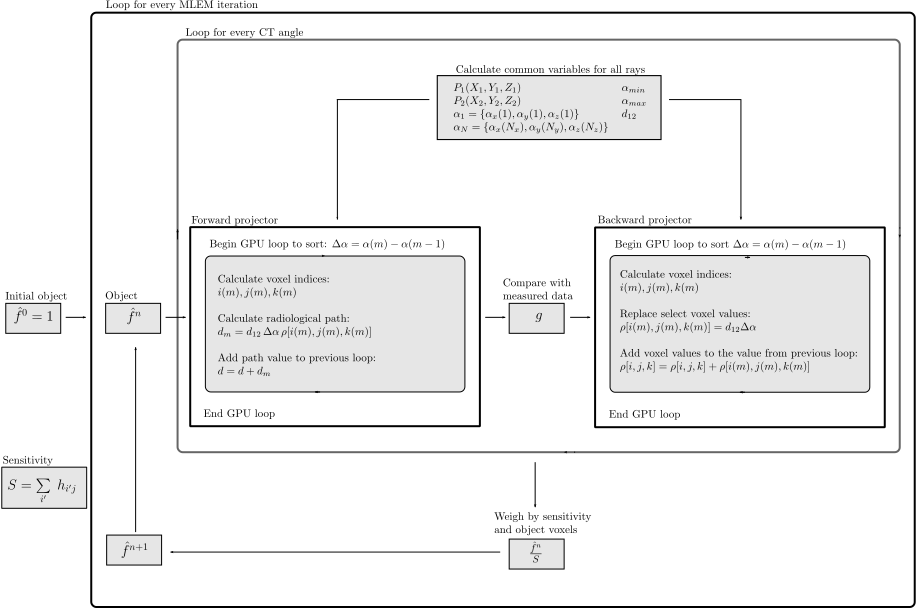
\includegraphics[scale=0.9]{siddon_flowchart.eps}
\caption{A flow chart of Siddon's algorithm implementation on CUDA}
\label{fig:siddon_algorithm_flow_chart}
\end{sidewaysfigure}
%
Figure~\ref{fig:siddon_algorithm_flow_chart} shows a flow chart of the implementation of Siddon's algorithm in CUDA.

\subsection{Forward and backward projector calculation}
The forward projector was implemented following Siddon's algorithm and Fig.~\ref{fig:siddon_algorithm_flow_chart}, where each x-ray originates from the x-ray point source and travels to the pixel center of each detector element.  The object voxel contribution to the ray was calculated using Eq.~\ref{eq:siddon_path}.  The treatment for the backward projector is very similar to the forward projector, with exception to an added CUDA function, \texttt{atomicAdd()}.  In the forward projection, each voxel index is calculated from the ray intersections with the planes of the object volume, and the contribution of voxel values to each ray is independent of other rays (i.e.\ the voxel values were read by the CUDA threads via read-only access, and tracing rays only involved reading the object voxel values).  However, in the backward projection the CUDA threads require that the object voxels need to have both read and write access, but since different ray needs access to the same voxel and the voxel value changes depending on the access sequence of the threads.  This requires an additional step of using \texttt{atomicAdd()} function that guarantees that access to the voxel value is sequential and without interference from other threads.  In other words, no other thread can access this address until the operation is complete.  For further information about this function please refer to the CUDA toolkit documentation~\cite{Cudatoolkit}.  Note because of this additional function, most of the bottleneck to the MLEM algorithm occurs here.  Another bottleneck occurs when $\{ \alpha \}$ is being sorted.

\subsection{Sensitivity calculation}

\begin{figure}[h]
\centering
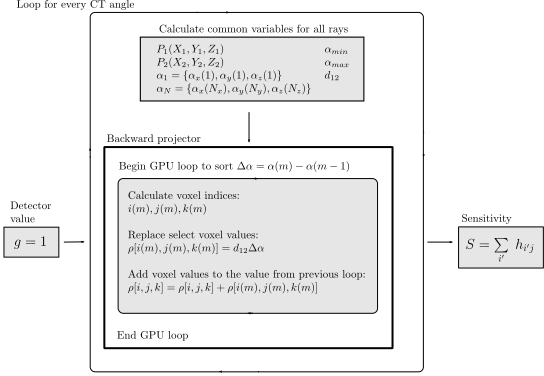
\includegraphics[scale=0.9]{siddon_flowchart_sensitivity.eps}
\caption{Flow chart for sensitivity calculation.}
\label{fig:sensitivityslices}
\end{figure}

The sensitivity used in the MLEM algorithm represents the contribution of all detector values at all projection angles on the object volume.  This was calculated by first setting all detector values to one, then back filling the object voxel values using the back projector for all scanned angles, shown in Fig~\ref{fig:sensitivityslices}.  Note that the sensitivity changes depending on the geometry of the CT system, number of object volume, number of detector pixels, and scan routine.  As a result, the sensitivity is always computed in the beginning of each reconstruction event.  However if one were to use a different data set while keeping geometry, object volume, and detector pixels constant, then sensitivity volume does not need to be recalculated and can speed up the reconstruction process.  Figure~\ref{fig:sensitivityslices} shows a few slices through the sensitivity volume using a set of CT parameters.
Figure~\ref{fig:reconstructedimage} shows the center slice of a reconstructed object after X iterations.

\subsection{Reconstruction results}
The prototype CT system has a XXX field of view, the x-ray magnification can be manually changed along with its optical magnification.  
\comment{
how to show the x-ray magnification, optical magnification as a function of FOV
}
\begin{figure}
\centering
placeholderimage[width=5cm, height=5cm]{reconstructedimage.png}
\label{fig:reconstructedimage}
\caption{reconstructed image slice after X iteration}
\end{figure}
\comment{show reconstruction image for maximum and minimum FOV?}

\subsection{Current algorithm limitations and assumptions}
Here are our assumptions and limitations in the algorithm we've implemented:
\begin{enumerate}
\item Each x-ray originate outside of the object volume, travels completely through the object.  So no ray will ever begin or end inside any voxel.
\item Object volume in each axis are divisible by 4, although it can be modified inside the code.
\item The number of detectors in both the trans-axial and axial directions can only be two to the power of $n$ (i.e. $2^n$ ).
\item Any ray traveling exactly along any voxel plane will not be calculated.
\end{enumerate}


%\comment{
%in the appendix explain the functions that are included in the algorithm\\
%explain how to checkout the repository (nvm)\\
%how to use the parameter file \\
%what are the outputs of each function (recon, forward, backward)
%}



